%\documentclass[a4paper,eqsecnum,twoside,aps,floatfix,notitlepage]{revtex4}



\documentclass[amsmath,amssymb,10pt,eqsecnum, twocolumn]{revtex4}
\usepackage{graphicx,float,subfloat}
\usepackage[breaklinks, colorlinks, citecolor=blue]{hyperref}
\usepackage{bm}% bold math

\usepackage{subfigure}
\usepackage{hyperref}

\newcommand{\Planck}{{\textit{Planck }}}
\newcommand{\SPT}{{\textit{SPT }}}
\newcommand{\CFHTLenS}{{\textit{CFHTLenS }}}
\newcommand{\CoRE}{{\textit{CoRE }}}
\newcommand{\WMAP}{{\textit{WMAP }}}
\newcommand{\Euclid}{{{\it Euclid}}}
\newcommand{\CAMB}{{\tt{CAMB }}}
\newcommand{\MGCAMB}{{\tt{MGCAMB }}}

%\newcommand{\vphi}[0]{{\color{green}{\delta\phi}}}
%\newcommand{\dlg}[0]{{\color{red}{\lp g}}}
\newcommand{\vphi}[0]{\delta\phi}
\newcommand{\lpa}[0]{\lp A}
\newcommand{\dlg}[0]{\lp g}

\newcommand{\depg}[0]{\ep g}
\newcommand{\virt}[0]{\hat{\delta}}
\newcommand{\Dvphi}[1]{\nabla_{#1}\vphi}
\newcommand{\DDvphi}[2]{\nabla_{#1}\nabla_{#2}\vphi}

\newcommand{\Dvvphi}[1]{\nabla_{#1}\virt\vphi}
\newcommand{\DDvvphi}[2]{\nabla_{#1}\nabla_{#2}\virt\vphi}

\newcommand{\tmat}[4]{\left( \begin{array}{cc} #1 & #2 \\ #3 & #4 \end{array}\right)}
\newcommand{\expec}[1]{\left\langle #1\right\rangle}
\newcommand{\half}[0]{\frac{1}{2}}
\newcommand{\cs}[3]{\Gamma^{#1}_{\,\,\,\, #2#3}}

\newcommand{\pd}[2]{\frac{\partial #1}{\partial #2}}
\newcommand{\ld}[0]{\mathcal{L}}
\newcommand{\md}[0]{\mathcal{M}}
\newcommand{\dd}[0]{\textrm{d}}
\newcommand{\defn}[0]{\equiv}
\newcommand{\diag}[0]{\textrm{diag}}
\newcommand{\qsubrm}[2]{{#1}_{\scriptsize{\textrm{#2}}}}
\newcommand{\qsuprm}[2]{{#1}^{\scriptsize{\textrm{#2}}}}
\newcommand{\qsubprm}[3]{{#1}^{\scriptsize{\textrm{#2}}}_{\scriptsize{\textrm{#3}}}}
 \newcommand{\subsm}[2]{{#1}_{\scriptscriptstyle{#2}}}

\newcommand{\supsm}[2]{{#1}^{\scriptscriptstyle{#2}}}
\newcommand{\symmb}[0]{\varrho}
\newcommand{\AW}[0]{A_{\mathcal{W}}}
\newcommand{\BW}[0]{B_{\mathcal{W}}}
\newcommand{\CW}[0]{C_{\mathcal{W}}}
\newcommand{\DW}[0]{D_{\mathcal{W}}}
\newcommand{\EW}[0]{E_{\mathcal{W}}}

\newcommand{\AP}[0]{A_{\mathcal{P}}}
\newcommand{\BP}[0]{B_{\mathcal{P}}}
\newcommand{\CP}[0]{C_{\mathcal{P}}}
\newcommand{\DP}[0]{D_{\mathcal{P}}}
\newcommand{\EP}[0]{E_{\mathcal{P}}}
\newcommand{\FP}[0]{F_{\mathcal{P}}}
\newcommand{\GP}[0]{G_{\mathcal{P}}}

\newcommand{\sol}[0]{\ld_{\scriptscriptstyle\{2\}}}

\newcommand{\tis}[0]{ {\theta}^{\scriptscriptstyle\rm{S}}}
\newcommand{\tisdot}[0]{ {\dot{\theta}}^{\scriptscriptstyle\rm{S}}}
\newcommand{\pis}[0]{ {\Pi}^{\scriptscriptstyle\rm{S}}}
\newcommand{\xis}[0]{ {\xi}^{\scriptscriptstyle\rm{S}}}
\newcommand{\xisdot}[0]{ {\dot{\xi}}^{\scriptscriptstyle\rm{S}}}
\newcommand{\xisddot}[0]{ {\ddot{\xi}}^{\scriptscriptstyle\rm{S}}}
\newcommand{\xisdddot}[0]{ {\dddot{\xi}}^{\scriptscriptstyle\rm{S}}}
\newcommand{\lcdm}[0]{$\Lambda$CDM}

\newcommand{\coup}[0]{\mathcal{Q}}
\newcommand{\vmkin}[0]{\mathcal{K}}



\newcommand{\newchap}[2]{\chapter{#1}
\markboth{\MakeUppercase{Chapter \thechapter.\ #2}}{}}
\newcommand{\nphiu}[1]{\nabla^{#1}\phi}
\newcommand{\nphid}[1]{\nabla_{#1}\phi}

\newcommand{\gbm}[1]{\bm{#1}}
\newcommand{\rbm}[1]{{\bf{#1}}}
\newcommand{\ci}[0]{\textrm{i}}
%\newcolumntype{V}{>{\centering\arraybackslash} m{.4\linewidth} }
\newcommand{\kin}[0]{{\mathcal{X}}}
\newcommand{\hct}[0]{\mathcal{H}}
\renewcommand{\figurename}{Figure}
\newcommand{\ep}[0]{{ {\delta}_{\scriptscriptstyle{\rm{E}}}}}
\newcommand{\lp}[0]{{ {\delta}_{\scriptscriptstyle{\rm{L}}}}}
\def\be{\begin{equation}}
\def\ee{\end{equation}}
\def\bea{\begin{eqnarray}}
\def\eea{\end{eqnarray}}
\def\bse{\begin{subequations}}
\def\ese{\end{subequations}}
\newcommand{\lied}[1]{\pounds_{#1}}

\newcommand{\sech}[0]{\textrm{ sech}}
% Planck style says this should be Fig. 1
\newcommand{\fref}[1]{{Fig.~\ref{#1}}}
\newcommand{\tref}[1]{{Table \ref{#1}}}
\newcommand{\secref}[1]{{section \ref{#1}}}
\newcommand{\Secref}[1]{{Section \ref{#1}}}
% PUT CATCH ON THE END OF SQUARE-ROOT SYMBOLS
\newcommand{\rsbb}[2]{#1_{\mathbb{#2}}}

\newcommand{\dg}[0]{\delta g}
\let\oldsqrt\sqrt
% it defines the new \sqrt in terms of the old one
\def\sqrt{\mathpalette\DHLhksqrt}
\def\DHLhksqrt#1#2{%
\setbox0=\hbox{$#1\oldsqrt{#2\,}$}\dimen0=\ht0
\advance\dimen0-0.2\ht0
\setbox2=\hbox{\vrule height\ht0 depth -\dimen0}%
{\box0\lower0.4pt\box2}}

\newcommand{\sbm}[2]{#1_{\mathbb{#2}}}

\newcommand{\comment}[1]{{\color{red}[#1]}}

 
\begin{document}

\title{Shaping the chameleon}
\author{Jonathan A. Pearson}
\email{j.pearson@nottingham.ac.uk}
\affiliation{School of Physics \& Astronomy, University of Nottingham, Nottingham, NG7 2RD, U.K.}	
\date{\today}

\maketitle




 
 
 
\section{Introduction}

The source density is $\rho(\rbm{x})$.  Different geometrical shapes of this source (such as ellipses, rectangles, triangles, etc) will yield different gravitational potentials, and will alter how the chameleon scalar responds.

The effective potential for the chameleon is
\bea
\label{eff-pot-cham}
\qsubrm{V}{eff} = \frac{\Lambda^5}{\phi} + \frac{\rho(\rbm{x})}{M}\phi + \half m^2\left( \phi - \phi_{\infty}\right)^2.
\eea
The equations governing the chameleon scalar and gravitational potential are
\bse
\label{eq:eom-cham-}
\bea
\nabla^2\phi = \frac{\dd \qsubrm{V}{eff}}{\dd\phi}.
\eea
\bea
\nabla^2\Phi = - \rho(\rbm{x})/2\qsubrm{M}{pl}^2
\eea
\ese
The force on a test particle, due to the gravitational and chameleon scalars are given by
\bea
\rbm{F}_{(\phi)} = - \tfrac{1}{M}\nabla\phi,\qquad \rbm{F}_{(\Phi)} = - \nabla\Phi.
\eea
The idea is to obtain the source-shape that maximises the force that a test particle will feel, that cannot be explained by forces of a purely gravitational origin.

We construct the function $\rho(\rbm{x})$ such that
\bea
\rho = \left\{ \begin{array}{cc} \rho_0 & \mbox{inside object}, \\ 0 & \mbox{outside object}. \end{array}\right.
\eea

\section{Explanation of numerical methods}
Discretize onto a grid. Using successive over relaxation and gradient flow.

The equations   implemented by our numerical methods are dimensionless. By setting
\bse
\bea
\phi = \sqrt{M\Lambda^5}\tilde{\phi},
\eea
\bea
\Phi = \frac{M}{\qsubrm{M}{Pl}^2}\sqrt{M\Lambda^5}\tilde{\Phi},
\eea
\bea
x^{\mu} = \sqrt{M}\left(M\Lambda^5\right)^{1/4}\tilde{x}^{\mu},
\eea
\bea
\tilde{m} = m M^{1/2}\left( \Lambda^5M\right)^{1/3},
\eea
\ese
the effective potential (\ref{eff-pot-cham}) becomes
\bea
\frac{M}{\sqrt{M\Lambda^5}}\qsubrm{V}{eff} = \frac{1}{\tilde{\phi}} + \rho \tilde{\phi} + \half \tilde{m}^2 \left( \tilde{\phi} - \tilde{\phi}_{\infty}\right)^2,
\eea
and the equations (\ref{eq:eom-cham-}) become
\bse
\bea
\tilde{\nabla}^2\tilde{\phi} = - \frac{1}{\tilde{\phi}^2} + \rho + \tilde{m}^2\left( \tilde{\phi} - \tilde{\phi}_{\infty}\right),
\eea
\bea
\tilde{\nabla}^2\tilde{\Phi} = - \half \rho.
\eea
\ese
The ratio of the  forces becomes
\bea
\frac{\left|\rbm{F}_{(\phi)} \right|}{\left|\rbm{F}_{(\Phi)} \right|} = \left( \frac{\qsubrm{M}{Pl}}{M}\right)^2\frac{\left| \tilde{\nabla}\tilde{\phi}\right|}{\left| \tilde{\nabla}\tilde{\Phi}\right|}
\eea
\subsection{Solving for the Chameleon}
We obtain the profile of the chameleon scalar around a given source profile $\rho(\rbm{x})$ using a gradient flow technique. This works by taking a initial guess for the scalar fields profile, and letting it ``relax'' into a profile which corresponds to a solution of the equation of motion.
\subsection{Solving Poisson's equation}
We have found conventional relaxation methods cumbersome and difficult to use for complicated shapes, mainly due to the nature of the boundary conditions (trying to put an ellipsoidal ``peg'' into a square ``box'' will always be problematic). We found it much more convenient, and incredibly computationally-cheap, to compute  the gravitational force, $\rbm{F}_{(\Phi)}$ at a given location, $\rbm{x}$, via the simple expression
\bea
\label{eq:sec:newt-grav-force}
\rbm{F}_{(\Phi)}(\rbm{x}) = - \frac{1}{8\pi \qsubrm{M}{Pl}^2}\sum_{i}m_i \frac{\rbm{x} - \rbm{x}_i}{\left| \rbm{x} - \rbm{x}_i\right|^3},
\eea
where $\{m_i,\rbm{x}_i\}$ are the mass and location of the $\qsuprm{i}{th}$ constituent of the source. One may feel uncomfortable at the explicitly discrete nature of the assumed distribution of the gravitating source. However, in any numerical solution of a field theory some kind of discretization scheme is used, and this places any fields onto the vertices of a lattice. This manifestly generates a discrete distribution: one aims to make the lattice spacing as small as possible, in order to best model a continuous field.



\section{Results}

\subsection{Properties of the gravitational force around different source geometries}
The Newtonian gravitational force (\ref{eq:sec:newt-grav-force}) is one of the simplest quantities one can compute, and its ``far-field'' properties are very well understood. However, we are interested in the ``near-field'' properties of the gravitational force: that is, how the gravitational force behaves near the source object.

\begin{figure}[!t]
      \begin{center}
{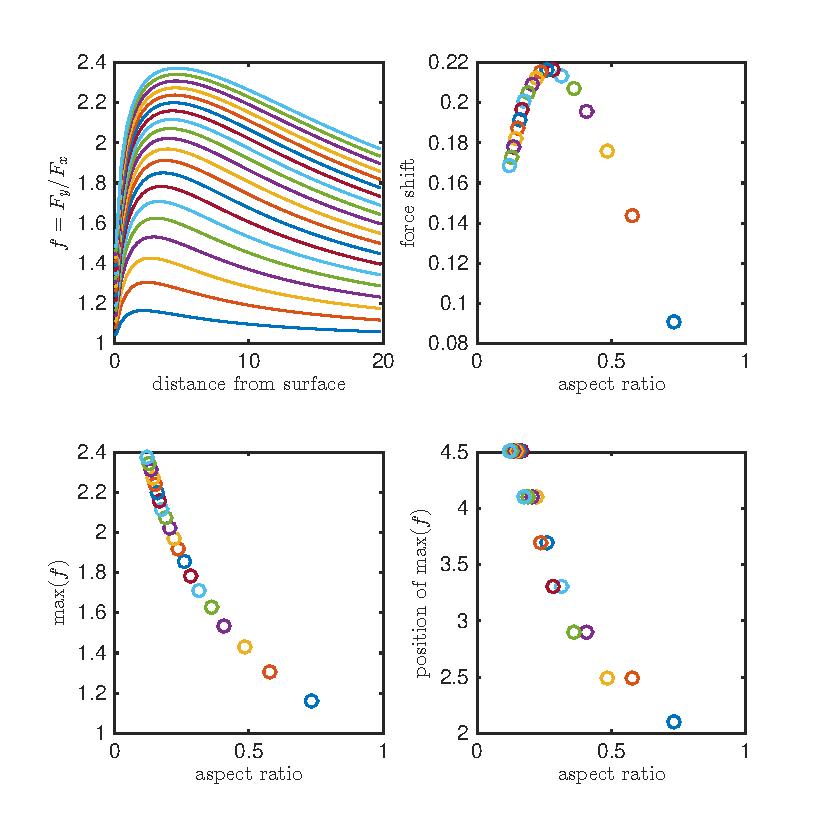
\includegraphics[scale=0.6,angle=0]{images/p2222}}
      \end{center}
\caption{ Interesting diagnostic quantities for the gravitational field around a squashed ellipse. The colour scheme between the panels is consistent. In the top-right panel we show the ratio $f$ of the force down the $x$- and $y$-axes as a function of distance from the surface; each colour corresponds to a different value of the aspect ratio of the ellipse. The actual values of the aspect ratios is given in the top-left panel, which shows the ``force shift''. This is the fractional difference between the maximum value of the force ratio, and the force ratio at the furthest distance from the surface shown. In the bottom-left panel we show the value of the maximum force ratio, as a function of the aspect ratio; in the bottom-right panel we show the position of the maximum force ratio. }\label{fig:squish-ellipse-grav}
\end{figure}

Creating a shape via
\bea
r(\theta) = \sum_{\ell=0}^n a_{\ell}P_{\ell}(\cos\theta)
\eea
In \tref{apple_coeffs} we give the values of the coefficients  $a_{\ell}$ required to generate the apple shape.
\begin{table}[!t]
\label{tab:priors}
\begin{center}
\begin{tabular}{|c|c|}  \hline 
Coefficient & Value \\ \hline 
$a_0$ & 0.3482169\\ \hline  
$a_1$ & 0.0969634 \\ \hline  
$a_2$ & -0.0450812 \\ \hline 
$a_3$ &  0.0346095\\ \hline 
$a_4$ & -0.0304927 \\ \hline  
$a_5$ &  0.0276200\\ \hline 
$a_6$ & -0.0245809\\ \hline 
$a_7$ & 0.0209728\\ \hline 
$a_8$ & -0.0168116\\ \hline  
$a_9$ & 0.0123419\\ \hline  
$a_{10}$ & -0.0079524\\ \hline  
$a_{11}$ & 0.0041198\\ \hline  
$a_{12}$ & -0.0013419\\ \hline   
\end{tabular}
\end{center}
\caption{Values of the coefficients in the Legendre expansion required to generate the ``apple'' shape.}
\label{apple_coeffs}
\end{table}%
\section{Discussion}
 
\end{document}
